% \documentclass{article}
% \usepackage{beamerarticle}
\documentclass{beamer}
% Beamer theme settings
\usetheme{Madrid}
\usecolortheme{default}
\usepackage{amsmath}
\usepackage{tikz}
\usepackage{mathtools}
\usepackage{hyperref}
\usetikzlibrary{intersections}
\usepackage{graphicx}
\usepackage{svg}
\usepackage{array}
\usepackage[table]{xcolor}


% Define commands for vectors
\newcommand{\va}{\mathbf{a}}
\newcommand{\vb}{\mathbf{b}}
\newcommand{\vc}{\mathbf{c}}
\newcommand{\vd}{\mathbf{d}}
\newcommand{\ve}{\mathbf{e}}
\newcommand{\vv}{\mathbf{v}}
\newcommand{\vu}{\mathbf{u}}
\newcommand{\vw}{\mathbf{w}}
\newcommand{\vx}{\mathbf{x}}
\newcommand{\vy}{\mathbf{y}}
\newcommand{\vz}{\mathbf{z}}
\newcommand{\N}{\mathbb{N}}
\newcommand{\Z}{\mathbb{Z}}
\newcommand{\R}{\mathbb{R}}
\newcommand{\Q}{\mathbb{Q}}
\newcommand{\E}{\mathbb{E}}
\newcommand{\PP}{\mathbb{P}}
\newcommand{\F}{\mathcal{F}}
\newcommand{\pw}{2^\Omega}
\newcommand{\rank}{\text{rank}}



\title[Lecture 9]{Random Variable, Expectation}
\author[Aprikyan, Tarkhanyan]{Hayk Aprikyan, Hayk Tarkhanyan}
\institute[ACA]{Armenian Code Academy}
\date{November 25, 2024}




\begin{document}

\begin{frame}
  \titlepage
\end{frame}


% slide 2: rv's
\begin{frame}{Random Variables}
Often we deal with situations involving some function \( X \) defined on a sample space \( \Omega \) of a given probability space \( (\Omega, \F, \PP) \). \pause For example, consider the experiment of throwing a fair dice, and assume we gamble on the outcome of this dice in such a way to:
\begin{itemize}
    \item win 1 if the outcome is a prime number,
    \item lose 1 in case of 4 or 6,
    \item and stay even if 1 shows up.
\end{itemize}
\pause Then our profit is a function \( X \) defined on \( \Omega \) where
\[ X(\omega) =
\begin{cases}
1, & \text{if } \omega \in \{2, 3, 5\}, \\
-1, & \text{if } \omega \in \{4, 6\}, \\
0, & \text{if } \omega = 1.
\end{cases}
\]
\pause The mapping \( X: \Omega \to \mathbb{R} \) is an example of a \textbf{discrete random variable}.

\textit{($X(\omega)$ is just a fancy way to denote a function: we could've written $f(x)$)}
\end{frame}



% slide 2: rv's
\begin{frame}{Random Variables}
In other words, if we have some quantity, the value of which is unknown, but we know the probabilistic distribution of its values (that is, with how much probability it will take a given value), that quantity is called a random variable.\pause 

\begin{block}{Definition}
    Let \( (\Omega, \F, \PP) \) be a probability space. If the function \( X : \Omega \to \mathbb{R} \) satisfies the condition
\[ \{\omega \in \Omega : X(\omega) \leq x\} \in \F \]
for all \( x \in \mathbb{R} \), then it is called a \textbf{Random Variable} (RV, rv).

\end{block}

\pause

Simply put, $X$ is the \textit{unknown} in the problem.


\end{frame}


% slide 2: rv's
\begin{frame}{Random Variables}
\begin{example}
    Some examples of random variables are:
    \begin{itemize}[<+->]
        \item the sum of two consecutive dice rolls,
        \item the number of goals in a football match,
        \item the difference between the scores of two teams,
        \item the number of children in a randomly selected family,
        \item the number of customers that enter a shop on a given day,
        \item the time until the bus arrives.
    \end{itemize}
\end{example}
\pause
\begin{block}{Definition}
    A random variable \( X \) is called \textbf{discrete} if the set of values of \( X \):
    \[ \text{Range}(X) = \{X(\omega) : \omega \in \Omega\} \]
    is finite or enumerable ($x_1, x_2, \dots$), i.e. is not an interval.

\end{block}

\end{frame}



% slide 2: rv's
\begin{frame}{Random Variables}
    
\begin{block}{Definition}
    For a discrete random variable \( X \), we define the \textbf{probability mass function (PMF)} of \( X \) by:
\[ p_X(x)= \PP(X = x), \]
or, equivalently,
\[p_X(x)= \PP(\{\omega \in \Omega : X(\omega) = x\}) \]

\end{block}\pause
$p_X(x)$ is simply the probability that $X$ takes the value $x$.
\pause
\begin{example}
    Let $X$ indicate the number on a fair die. Then its PMF is:
    \[ 
    p_X(x)=\begin{cases}
        \frac{1}{6}, &x\in\{1,2,3,4,5,6\},\\
        0,&\text{otherwise}
    \end{cases}
    \]
\end{example}

\end{frame}


% slide 2: rv's
\begin{frame}{Random Variables}

    If $\operatorname{Range}(X) = \{x_1, x_2, \dots\}$, we denote:
    \[
    p_k = p_X(x_k) = \PP(X=x_k),
    \]
    \pause and can represent the PMF of $X$ with a table:
   
\begin{table}[h]
\centering
\begin{tabular}{|c|c|c|}
\hline
$x$ & $\PP(X=x)$ \\
\hline
$x_1$ & $p_1$ \\
$x_2$ & $p_2$ \\
\vdots & \vdots \\
\hline
\end{tabular}
\end{table}


\end{frame}

% slide 2: rv's
\begin{frame}{Random Variables}
    
\begin{block}{Definition}
    For any random variable \( X \), we define the \textbf{cumulative distribution function (CDF)} of \( X \) by:
\begin{center}
    $F_X(x) = \PP(X \leq x)$
\end{center}% or, equivalently,
% \[F_X(x)= \PP(\{\omega \in \Omega : X(\omega) \le x\}) \]

\end{block}\pause
\begin{example}
    Let $X$ indicate the number on a fair die. Then for any number $x >6$, $F_X(x) = \PP(X \le x) = $ \pause $ 1$. \pause For any $x\in(5,6)$,  $F_X(x) = \PP(X \le x) = $ \pause $ \frac{5}{6}$. \pause What about $F_X(6)$? \pause $F_X(6) = 1$, too. 
\end{example}

\end{frame}

% slide 2: rv's
\begin{frame}{Random Variables}
    \begin{example}
        Continuing this way, we get:
    \[ F_X(x)=\begin{cases}
    0,&x<1,\\
    \frac{1}{6},&1\le x<2,\\
    \frac{2}{6},&2\le x<3,\\
    \frac{3}{6},&3\le x<4,\\
    \frac{4}{6},&4\le x<5,\\
    \frac{5}{6},&5\le x<6,\\
    1,&x\ge6
    \end{cases}
    \]
    
    \end{example}

\end{frame}


% slide 2: rv's
\begin{frame}{Random Variables}


\begin{block}{Properties}
\begin{itemize}[<+->]
    \item $0 \leq F_X(x) \leq 1, \; \text{for any } x \in \mathbb{R}$
\item $F_X(x) \text{ is a non-decreasing function}$
\item $\lim\limits_{x\to-\infty} F_X(x) = 0$\\
$\lim\limits_{x\to+\infty} F_X(x) = 1 $

\end{itemize}

\end{block}

\pause 

\begin{figure}
    \centering
    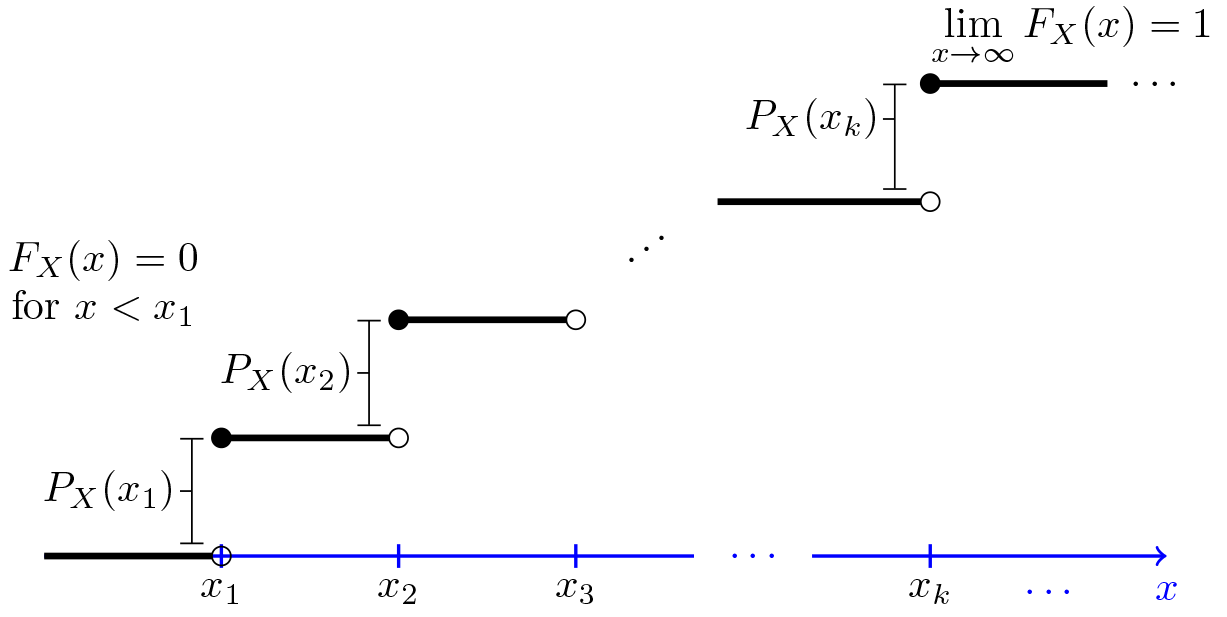
\includegraphics[width=0.7\linewidth]{cdf_typical.png}
\end{figure}
\end{frame}


% slide 2: rv's
\begin{frame}{Random Variables}
    What if a RV takes too many values?\pause

    For example, let $X(\omega)$ denote the minutes until the bus arrives, ($\omega$ can be time/coordinates/bus number). \pause $X(\omega)$ can be any real number between $0$ and, say, $60$. Recall that for any $x\in[0,60],\,$ $\PP(X=x)=0$.
    
    \pause What can we say about $X$?\pause

\begin{block}{Definition}
    We say that \( X \) is a \textbf{continuous random variable} if there exists a nonnegative function \( f(x) \) such that:
\[ F_X(x) = \PP(X \leq x) = \int_{-\infty}^{x} f(t) \, dt \]
\pause The function \( f \) is called the \textbf{probability density function (PDF)} of the random variable \( X \).

\end{block}\pause
The PDF of a continuous RV is essentially the same as the PMF of a discrete RV.

\end{frame}


% slide 2: rv's
\begin{frame}{Random Variables}
    
\begin{example}
    Some examples of continuous random variables are:
    \begin{itemize}[<+->]
        \item the marathon time of a given runner,
        \item the number of minutes until a bus arrives,
        \item the height of a randomly selected person,
        \item the stocks of Apple tomorrow,
        \item the $x$-coordinate of a randomly selected point on the $(x,y)$-plane.
    \end{itemize}
\end{example}

\pause 

Roughly speaking, every unknown thing is a random variable. If its value can be any number in a given  interval, we call it \textit{continuous}, otherwise \textit{discrete}.

\end{frame}


% slide 2: rv's
\begin{frame}{Random Variables}
Just like the density of an object measures the concentration of mass (per unit volume), the probability density function captures the density of \textit{probability} at point $x$:

\[
f_X(x)=\lim_{\Delta x \to 0} \frac{\PP(x < X \leq x+\Delta x)}{\Delta x}
\]
 \pause
      \begin{center}

    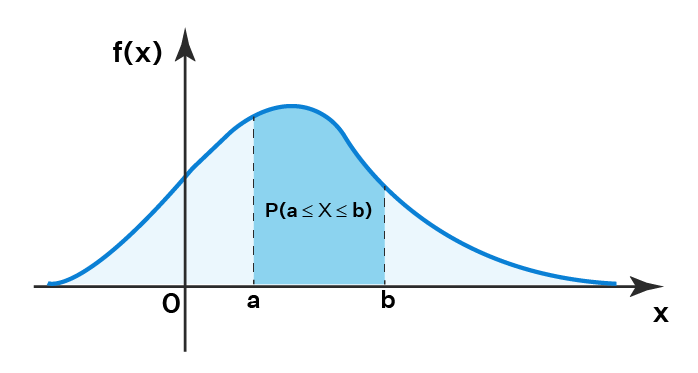
\includegraphics[width=0.75\textwidth, height=\textheight, keepaspectratio]{pdf.png}
  \end{center}
 
\end{frame}


% slide 2: rv's
\begin{frame}{Random Variables}
\begin{block}{Properties}
    \begin{enumerate}[<+->]
        \item $f_X(x) \geq 0 \quad \text{for all } x \in \mathbb{R}$
        \item $\displaystyle\int_{-\infty}^{\infty} f_X(x) \, dx = 1$
        \item If $F_X$ is continuous at $x$, $F_X'(x)=f_X(x)$
        \item $\displaystyle\PP(a < X \leq b) = F_X(b) - F_X(a) = \int_{a}^{b} f_X(x) \, dx$
        \item $\displaystyle\PP(X=a) =\PP(X\le a)-\PP(X<a)=F(a)-\lim_{\substack{\tilde{a}\to a\\\tilde{a} < a}} F(\tilde{a})$
        % \item $\displaystyle\text{More generally, for a set } A, \quad \PP(X \in A) = \int_{A} f_X(x) \, dx$
    \end{enumerate}
\end{block}
\end{frame}



% slide 2: rv's
\begin{frame}{Random Variables}
\begin{example}
    Ani chooses a random real number $X$ uniformly from the interval $[a,b]$.
\newline
\newline 
    {\small By "uniformly" we mean that for any two intervals of the same length (e.g. $(1.3, 1.5)$ and $(4.7, 4.9)$) $X$ can belong to them with the same probability.}
\newline 

    \pause Let's find the CDF and PDF of $X$.\pause

\end{example}

\pause
For $x<a$, $F_X(x)=\PP(X\le x)=0$,\pause

\medskip

For $x \ge b$, $F_X(x)=\PP(X \le x)=1$,\pause

\medskip

For $a\le x \le b$, we have:
\[F_X(x)=\PP(X\le x)=\PP(X\in[a,x])=\dfrac{x-a}{b-a}
\]
\end{frame}



% slide 2: rv's
\begin{frame}{Random Variables}
      \begin{center}

    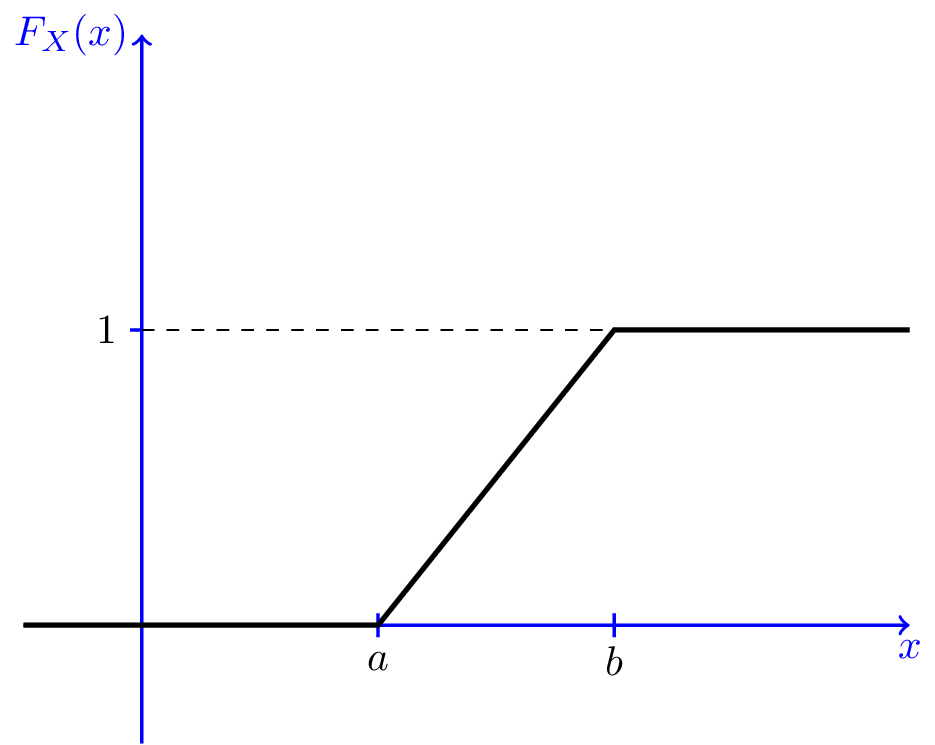
\includegraphics[width=0.6\textwidth, height=\textheight, keepaspectratio]{ex_cdf.png}
  \end{center}
\pause
Thus, 
\begin{equation*}
F_X(x) = \left\{
\begin{array}{l l}
0 & \quad \text{for } x < a \\
\frac{x-a}{b-a} & \quad \text{for }a \leq x \leq b\\
1 & \quad \text{for } x > b
\end{array} \right.
\end{equation*}

\end{frame}



% slide 2: rv's
\begin{frame}{Random Variables}
To find $f_X(x)$, we take the derivative of $F_X(x)$:
\begin{equation*}
f_X(x) = \left\{
\begin{array}{l l}
\frac{1}{b-a} & \quad a < x < b\\
0 & \quad x < a \text{ or } x > b
\end{array} \right.
\end{equation*}\pause
      \begin{center}

    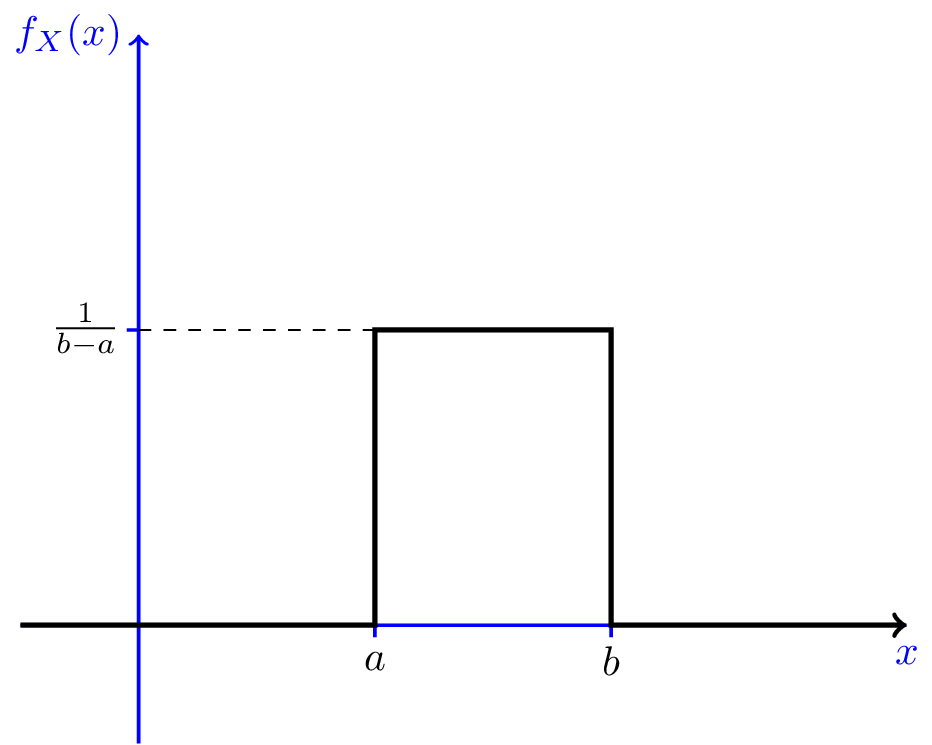
\includegraphics[width=0.6\textwidth, height=\textheight, keepaspectratio]{ex_pdf.png}
  \end{center}

\end{frame}


% slide 2: rv's
\begin{frame}{Random Variables}
\begin{block}{Definition}
   
Two random variables are said to be \textbf{identically distributed} if their
CDFs are equal.

    
\end{block}\pause

\begin{block}{Remark}
    Two random variables may be identically distributed but \textit{not equal}.
\end{block}
\begin{example}
    Say we toss a fair coin. $X$ and $Y$ are RVs such that:
    \[
X(\omega)=\begin{cases}
    0,&\omega=\textbf{H},\\
    1,&\omega=\textbf{T},
\end{cases}\qquad
Y(\omega)=\begin{cases}
    1,&\omega=\textbf{H},\\
    0,&\omega=\textbf{T},
\end{cases}\]
\pause They both have the save PMFs:
\begin{center}
    $p_X(0)=p_X(1)=p_Y(0)=p_Y(1)=\frac{1}{2}\pause\qquad \text{but }X\ne Y$
\end{center}
\end{example}

\end{frame}


% slide 3: indep
\begin{frame}{Independence}
    Given a probability space \( (\Omega, \F, \PP) \), recall that two events \( A, B \in \F \) are called independent if \( \PP(A \cap B) = \PP(A)\PP(B) \). We now extend the concept of independence from events to random variables.\pause

    Let $(\Omega, \F, \PP)$ be a probability space, and $X, Y$ are any two (discrete or continuous) random variables defined on it.\pause

\begin{block}{Definition}
   \( X \) and \( Y \) are called \textbf{independent} if
\[ \PP(X \le x, Y \le y) = \PP(X \le x)\PP(Y \le y) \quad \text{for all } x,y\in\R\]
\end{block}
\pause In case of discrete random variables,

% \pause

\begin{block}{Theorem}
  Two \textit{discrete} random variables \( X \) and \( Y \) are independent if and only if
\begin{center}
    $\PP(X = x, Y = y) = \PP(X = x)\PP(Y = y)$
\end{center}
for all \( x, y \in \mathbb{R} \).
    
\end{block}


\end{frame}


% slide 3: indep
\begin{frame}{Independence}
    Similarly,

\begin{block}{Definition}
Random variables \( X_1, X_2, \dots, X_n \) are called \textbf{independent} if
\[ \PP(X_1 \le x_1, X_2 \le x_2, \dots, X_n \le x_n) =\prod_{i=1}^n \PP(X_i \le x_i)\]
for all $x_1,\dots,x_n\in\R$.
\end{block}
% \pause In case of discrete random variables,

\pause

\begin{block}{Theorem}
  $n$ \textit{discrete} random variables \( X_1, X_2, \dots, X_n \) are independent if and only if
  \begin{center}
      $\PP(X_1 = x_1, X_2 = x_2, \dots, X_n = x_n) =\prod_{i=1}^n \PP(X_i =x_i)$
  \end{center}
for all $x_1,\dots,x_n\in\R$.
\end{block}


\end{frame}





% slide 4: E
\begin{frame}{Expected Value}
\begin{figure}
    \centering
    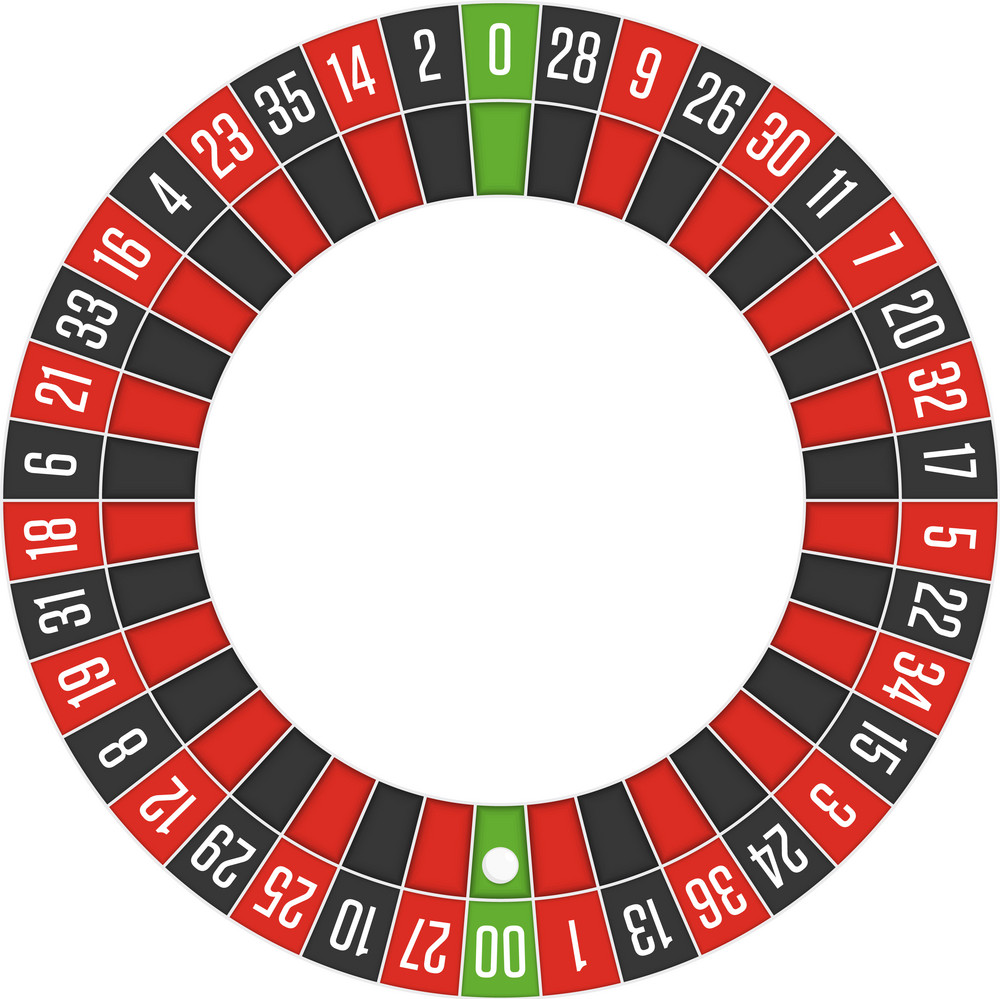
\includegraphics[width=0.3\linewidth]{roulette.png}
    % \caption{Enter Caption}
    % \label{fig:enter-label}
\end{figure}
Suppose you are playing roulette, with numbers 1 to 38 on it. You bet a number and spin it. \pause Say you have picked the number 8 and bet \$1. \pause
\begin{itemize}[<+->]
    \item If it falls on 8, you win \$35,
    \item Otherwise, you lose \$1.
\end{itemize}
\pause Would you play this game?
\pause \vspace{0.3em}
What if instead of \$35, you won \$150 if it fell on 8? \pause How about \$38.01?

\end{frame}



% slide 4: E
\begin{frame}{Expected Value}

    \begin{block}{Definition}
      The \textbf{expectation} or the \textbf{expected value}, of a continuous random variable \( X \), denoted by \( \mathbb{E}(X) \), is defined by
\[ \mathbb{E}(X) = \int_{-\infty}^{\infty} x \cdot f_X(x) \, dx \]

      The \textbf{expectation} or the \textbf{expected value}, of a discrete random variable \( X \), denoted by \( \mathbb{E}(X) \), is defined by
\[ \mathbb{E}(X) = \sum_{x_i} x_i\cdot \PP(X=x_i) \]

    \end{block}

\pause
    In words, the expected value of discrete random variable $X$ is a weighted
average of the possible values that $X$ can take on, each value being
weighted by the probability that $X$ assumes it.

\end{frame}


% slide 4: E
\begin{frame}{Expected Value}

We have seen that if $X$ is a random variable, so is $X^2$, $X^3$ or $\sin{X}$. \pause In general,
\begin{block}{Definition}
If $X$ is a random variable and $g(x)$ is a continuous function, then $g(X)$ is a random variable too.
\end{block}
\pause

    \begin{block}{Theorem}
If \( X \) is a continuous random variable, then for any continuous function \( g \),
\[\mathbb{E}(g(X)) = \int_{-\infty}^{\infty} g(x) \cdot f_X(x) \, dx \]

If \( X \) is a discrete random variable, then for any continuous function \( g \),
\[\mathbb{E}(g(X)) = \sum_{x_i} g(x_i)\cdot \PP(X=x_i)  \]

    \end{block}


\end{frame}





% slide 4: E
\begin{frame}{Expected Value}
\begin{block}{Properties}
    \begin{enumerate}[<+->]
        \item If $a$ and $b$ are constants, then
        \[
        \E(aX+b)=a\E(X)+b
        \]
        \item $\E(X+Y)=\E(X)+\E(Y)$
        \item $\E(X_1+X_2+\dots+X_n)=\E(X_1)+\E(X_2)+\dots+\E(X_n)$
        \item If $X\ge Y$, then $\E(X)\ge \E(Y)$
    \end{enumerate}
\end{block}
\pause
% \begin{figure}
%     \centering
%     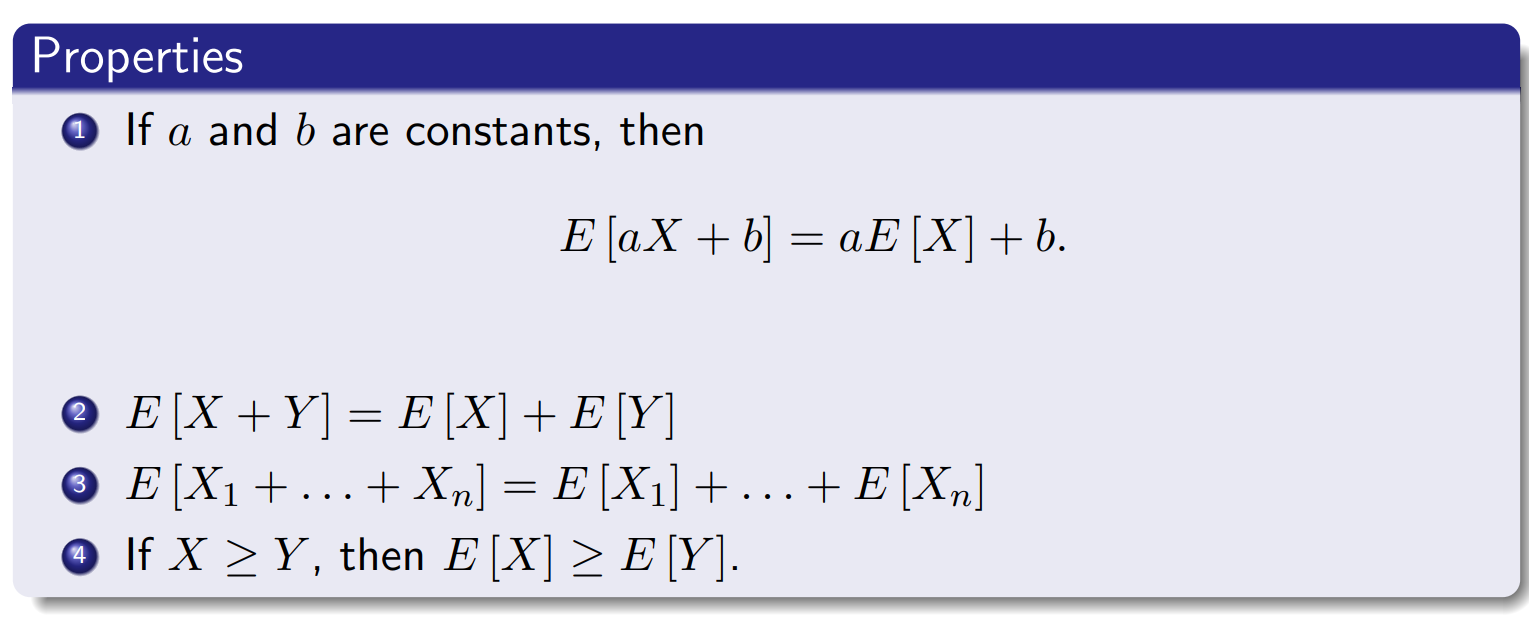
\includegraphics[width=1\linewidth]{var1.png}
% \end{figure}
% \pause
\begin{block}{Theorem}
    If \( X \) and \( Y \) are independent random variables, then
\[\mathbb{E}(XY) = \mathbb{E}(X)\cdot \mathbb{E}(Y) \]

\end{block}
The converse is not necessarily true.

\end{frame}




% % slide 3: var
% \begin{frame}{Variance}
% \begin{figure}
%     \centering
%     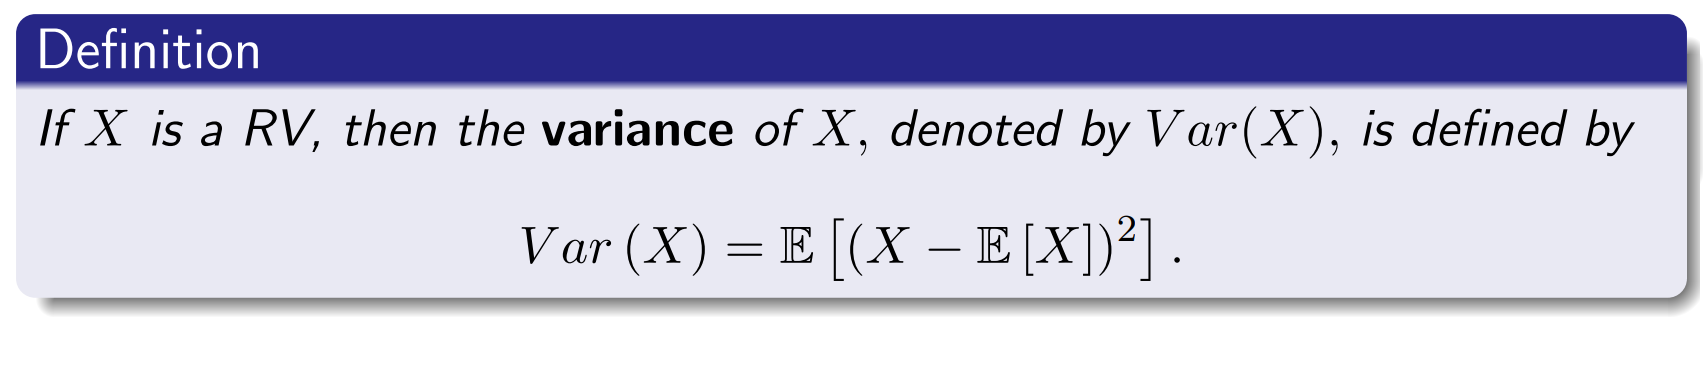
\includegraphics[width=1\linewidth]{var2.png}
    
    
% \end{figure}
% \pause\begin{figure}
%     \centering
%     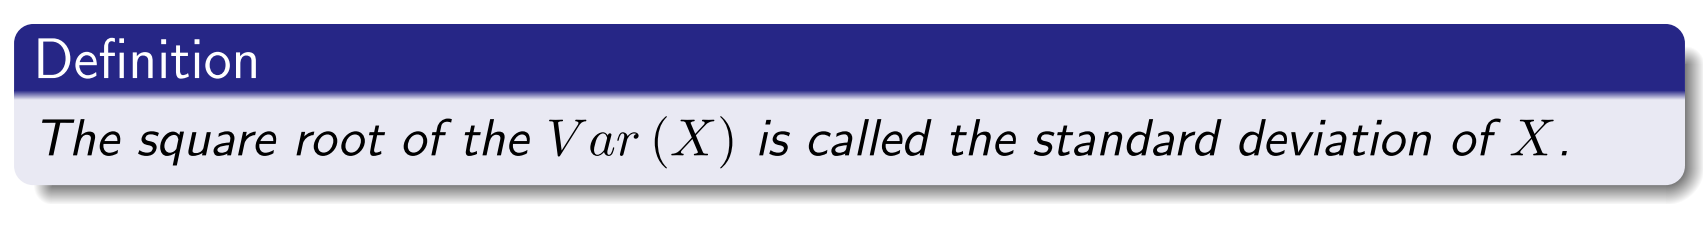
\includegraphics[width=1\linewidth]{var3.png}
    
    
% \end{figure}

% \pause
% \begin{figure}
%     \centering
%     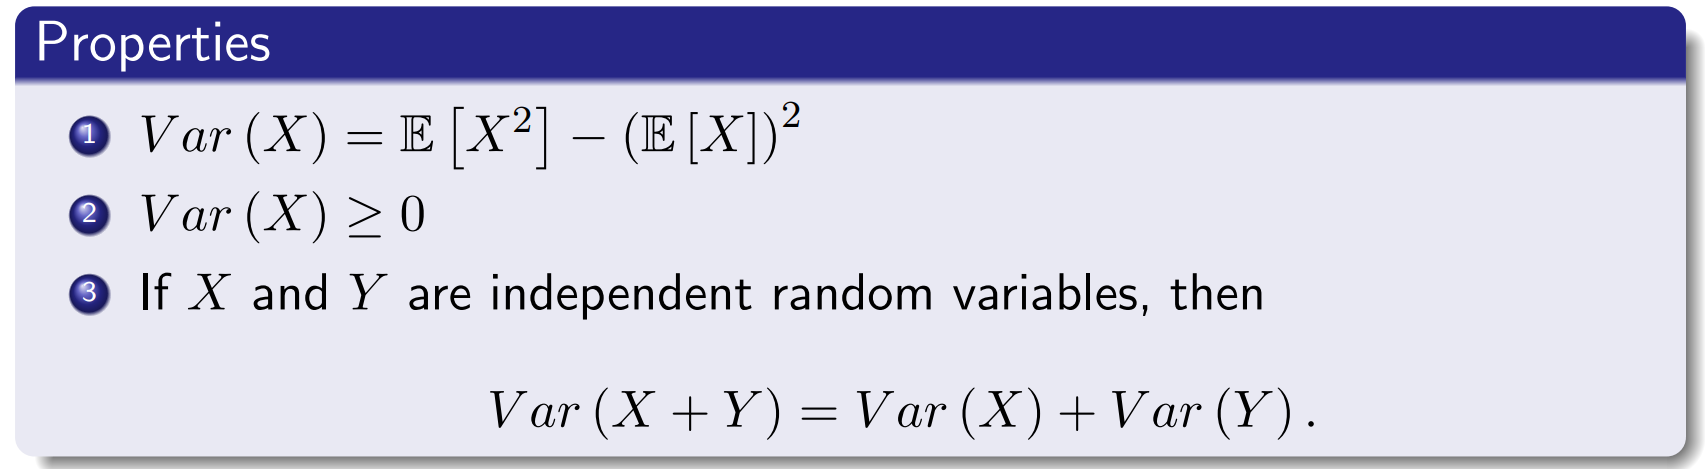
\includegraphics[width=1\linewidth]{var4.png}
    
    
% \end{figure}
% \end{frame}







% % slide __: covariance
% \begin{frame}{Covariance}
% % \begin{example}
%     Consider the following example: \pause Lilit and Aram are playing Texas hold’em.
    
%     \pause Lilit is looking at her 2 cards, which are:
%       \begin{center}

%     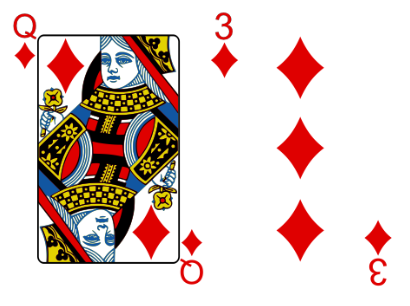
\includegraphics[width=0.2\textwidth, height=\textheight, keepaspectratio]{lilit.png}
%   \end{center}
% She wonders how many more \textbf{diamonds} there are in the community cards.\pause

% Aram, on the other hand, has the following cards:
%       \begin{center}

%     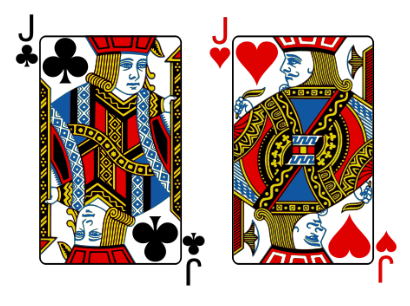
\includegraphics[width=0.2\textwidth, height=\textheight, keepaspectratio]{aram.png}
%   \end{center}
% He is interested in the number of \textbf{jacks} among the community cards.\pause

% Both Lilit and Aram are interested in the same random process, yet different RVs. \textit{How much} are those RVs related?
% % \end{example}
% \end{frame}


% % slide __: covariance
% \begin{frame}{Covariance}
%    \begin{block}{Definition}
%        The \textbf{covariance} between random variables \( X \) and \( Y \) is defined by
% \[ \text{Cov}(X, Y) = \mathbb{E}\big((X - \mathbb{E}(X)(Y - \mathbb{E}(Y)\big) \]

%    \end{block}\pause
%    Note that the formula for covariance can be simplified to
% \[ \text{Cov}(X, Y) = \mathbb{E}(XY) - \mathbb{E}(X)\mathbb{E}(Y) \]

% \pause Covariance shows how much the linear growth of one RV is related to the linear growth of the other RV. It is very similar to the concept of dot product of two vectors.
    
% \end{frame}


% % slide __: covariance
% \begin{frame}{Covariance}
%    \begin{block}{Properties}
%        \begin{enumerate}[<+->]
%            \item \( \text{Cov}(X, Y) = \text{Cov}(Y, X) \),
% \item \( \text{Cov}(X, X) = \text{Var}(X) \),
% \item  \( \text{Cov}(a \cdot X, Y) = a \cdot \text{Cov}(X, Y) \),
% \item  \(\displaystyle \text{Cov}\left(\sum_{i=1}^{n} X_i, \sum_{j=1}^{k} Y_j\right) = \sum_{i=1}^{n}\sum_{j=1}^{k} \text{Cov}(X_i, Y_j) \),
% \item  \(\displaystyle \text{Var}\left(\sum_{i=1}^{n} X_i\right) = \sum_{i=1}^{n} \text{Var}(X_i) + 2 \sum_{i: i<j} \text{Cov}(X_i, X_j) \),
% \item If $X$ and $Y$ are independent, $\text{Cov}(X, Y)=0$ (converse isn't true).

%        \end{enumerate}
%    \end{block}
%    \pause 
%    $\text{Cov}(X, Y)$ can be \textit{any} number (positive/negative, large/small, zero, etc). What if we want a normalized, universal method to measure the relatedness level of two RVs?
    
% \end{frame}

% % slide __: corr
% \begin{frame}{Correlation}

%    \begin{block}{Definition}
%        For two non-constant ($\text{var}(X), \text{var}(Y) \ne 0$) random variables \( X \) and \( Y \), the \textbf{correlation} (or \textbf{Pearson correlation coefficient}) between them is defined as:
% \[ \rho(X,Y)=\text{Corr}(X, Y) = \frac{\text{Cov}(X, Y)}{\sqrt{\text{Var}(X) \cdot \text{Var}(Y)}} \]

%    \end{block}
%    \pause
%    \begin{block}{Properties}
% \begin{enumerate}
%     \item \( \rho(X, Y) = \rho(Y, X) \),
%     \item \( |\rho(X, Y)| \leq 1 \),
%     \item \( Y = aX + b \) for some constants \( a, b \) if and only if \( \rho(X, Y) = \pm 1 \).
% \end{enumerate}
%    \end{block}
    
% \end{frame}



% % slide 4: derivative
% \begin{frame}{Derivative}
%       \begin{center}

%     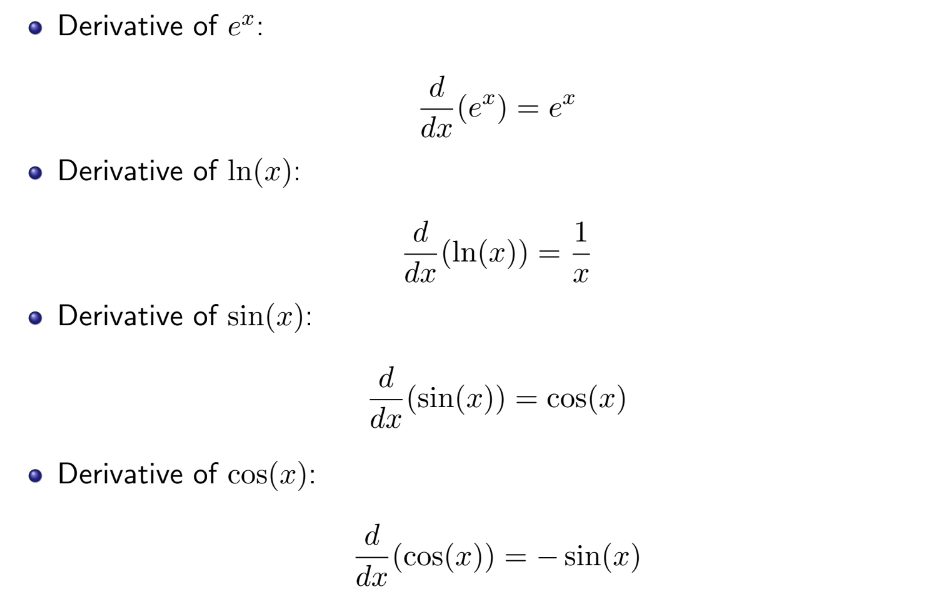
\includegraphics[width=0.9\textwidth, height=\textheight, keepaspectratio]{der2.png}
%   \end{center}
% \end{frame}



% % slide 5: extrema
% \begin{frame}{Extrema of a Function}

% % \begin{center}
% \begin{exampleblock}{Example}
%     Which points are the local extremum points of the following functions? \\ \bigskip
% % \\\includesvg[ width=0.31\textwidth, keepaspectratio]{image-295}\pause 
%  \includesvg[ width=0.31\textwidth, keepaspectratio]{image-296}\pause
%  \includesvg[ width=0.31\textwidth, keepaspectratio]{image-297}\pause
%  \includesvg[ width=0.31\textwidth, keepaspectratio]{image-290}
% \end{exampleblock}
%   % \end{center}
% \pause
% \begin{block}{Theorem}
% If a function \(f\) is continuous on a \textit{closed interval} \([a, b]\), then \(f\) has both a global maximum and a global minimum on \([a, b]\).
    
% \end{block}

  
% \end{frame}


\end{document}
